% Fig 1 — CAFRL architecture (the hypothesis under test), standalone TikZ.
% Compile: pdflatex -interaction=nonstopmode fig1_architecture.tex
% Faithful to the as-built model (docs/phases/phase{2,3}-asbuilt.md):
% three streams; compression estimator conditions the band gate + fusion gate
% via zero-init FiLM (estimated arm); z_freq = pre-CMAM frequency tap (excludes
% F_spat) feeds the GRL discriminator; SplitBN + curriculum noted in the caption.
\documentclass[tikz,border=10pt]{standalone}
\usetikzlibrary{positioning,arrows.meta,calc}

\definecolor{spat}{HTML}{2A78D6}   % spatial stream
\definecolor{freq}{HTML}{E34948}   % frequency streams
\definecolor{estc}{HTML}{4A3AA7}   % estimator / conditioning
\definecolor{advc}{HTML}{52514E}   % adversary
\definecolor{ink}{HTML}{0B0B0B}
\definecolor{ink2}{HTML}{52514E}
\definecolor{muted}{HTML}{898781}

\begin{document}
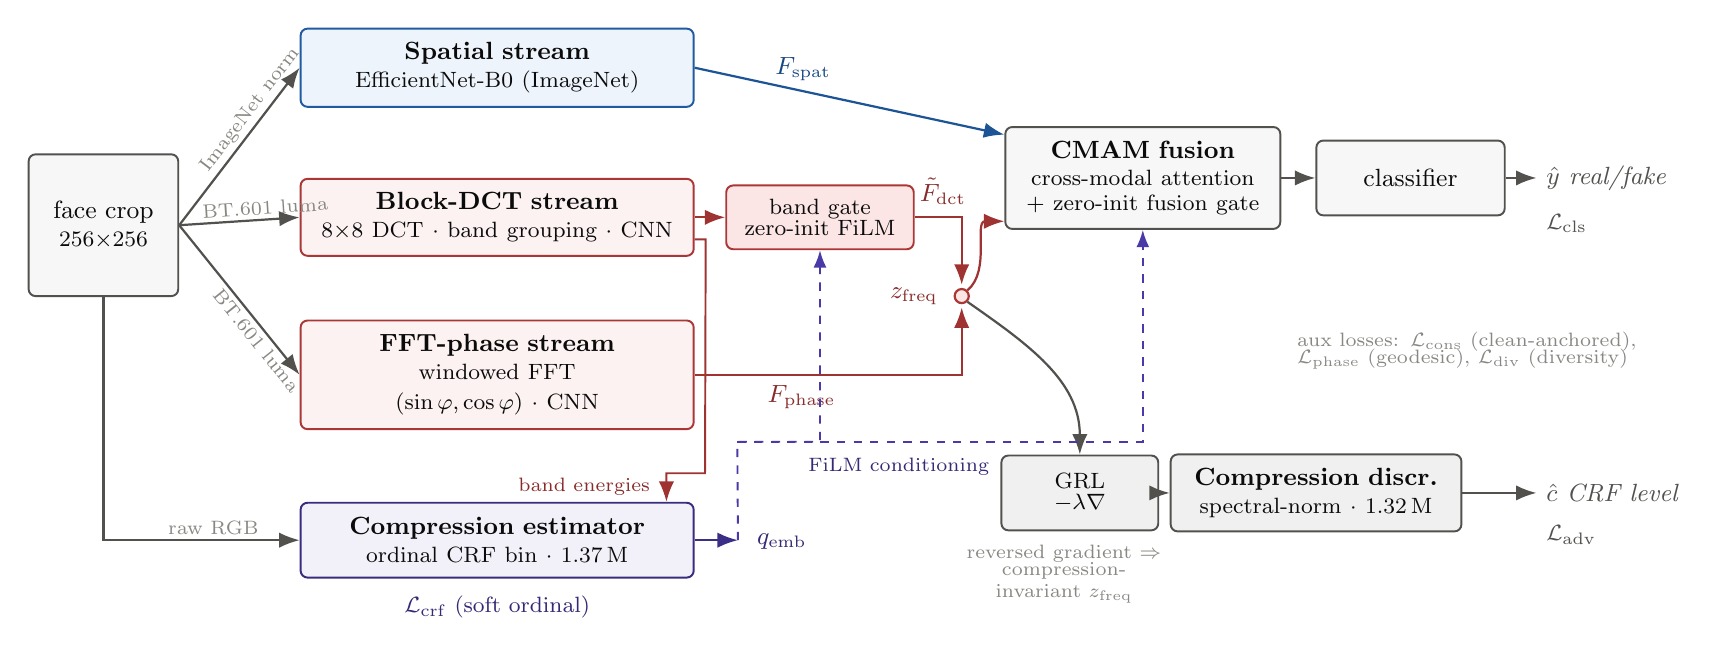
\begin{tikzpicture}[
  font=\small,
  every node/.style={text=ink},
  block/.style={draw, rounded corners=2.5pt, align=center, minimum height=9.5mm, inner xsep=7pt, inner ysep=5pt, line width=0.7pt},
  spatblock/.style={block, draw=spat!75!black, fill=spat!8},
  freqblock/.style={block, draw=freq!75!black, fill=freq!7},
  estblock/.style={block, draw=estc!75!black, fill=estc!7},
  advblock/.style={block, draw=advc, fill=black!6},
  fuseblock/.style={block, draw=ink2, fill=black!3},
  gate/.style={block, draw=freq!75!black, fill=freq!14, inner xsep=4pt, minimum height=8mm, font=\footnotesize},
  flow/.style={-{Latex[length=2.6mm]}, line width=0.8pt, draw=ink2},
  cond/.style={-{Latex[length=2.2mm]}, line width=0.7pt, draw=estc, dashed},
  elab/.style={font=\scriptsize, text=muted, inner sep=1.5pt},
  olab/.style={font=\small\itshape, text=ink2},
  loss/.style={font=\footnotesize, text=ink2},
]

% ---------------------------------------------------------------- input ----
\node[block, draw=ink2, fill=black!3, minimum width=1.9cm, minimum height=1.8cm, align=center] (input) at (0,0.4)
  {face crop\\[-1pt]{\footnotesize $256{\times}256$}};

% --------------------------------------------------------------- streams ---
\node[spatblock, text width=4.5cm] (spatial) at (5.0, 2.4)
  {\textbf{Spatial stream}\\[-1pt]{\footnotesize EfficientNet-B0 (ImageNet)}};
\node[freqblock, text width=4.5cm] (dct) at (5.0, 0.5)
  {\textbf{Block-DCT stream}\\[-1pt]{\footnotesize $8{\times}8$ DCT $\cdot$ band grouping $\cdot$ CNN}};
\node[freqblock, text width=4.5cm] (phase) at (5.0, -1.5)
  {\textbf{FFT-phase stream}\\[-1pt]{\footnotesize windowed FFT $(\sin\varphi,\cos\varphi)$ $\cdot$ CNN}};
\node[estblock, text width=4.5cm] (est) at (5.0, -3.6)
  {\textbf{Compression estimator}\\[-1pt]{\footnotesize ordinal CRF bin $\cdot$ 1.37\,M}};

% ------------------------------------------------------------- band gate ---
\node[gate, text width=2.1cm] (bandgate) at (9.1, 0.5)
  {band gate\\[-2pt]zero-init FiLM};

% -------------------------------------------------------- z_freq junction --
\node[circle, draw=freq!75!black, fill=freq!14, inner sep=1.8pt, line width=0.8pt] (zfreq) at (10.9, -0.5) {};
\node[olab, text=freq!60!black, anchor=east] at ($(zfreq.west)+(-0.08,0)$) {$z_{\mathrm{freq}}$};

% ----------------------------------------------------------------- fusion --
\node[fuseblock, text width=3.0cm] (fusion) at (13.2, 1.0)
  {\textbf{CMAM fusion}\\[-1pt]{\footnotesize cross-modal attention}\\[-2pt]{\footnotesize + zero-init fusion gate}};
\node[block, draw=ink2, fill=black!3, text width=1.9cm] (clf) at (16.6, 1.0) {classifier};
\node[olab, anchor=west] (yout) at (18.2, 1.0) {$\hat{y}$ real/fake};
\node[loss, anchor=north west] at ($(yout.south west)+(0,-0.05)$) {$\mathcal{L}_{\mathrm{cls}}$};

% -------------------------------------------------------------- adversary --
\node[advblock, text width=1.5cm, font=\footnotesize] (grl) at (12.4, -3.0)
  {GRL\\[-2pt]$-\lambda\nabla$};
\node[advblock, text width=3.2cm] (disc) at (15.4, -3.0)
  {\textbf{Compression discr.}\\[-1pt]{\footnotesize spectral-norm $\cdot$ 1.32\,M}};
\node[olab, anchor=west] (cout) at (18.2, -3.0) {$\hat{c}$ CRF level};
\node[loss, anchor=north west] at ($(cout.south west)+(0,-0.05)$) {$\mathcal{L}_{\mathrm{adv}}$};

% ------------------------------------------------------------ input edges --
\draw[flow] (input.east) -- (spatial.west)
  node[elab, pos=0.68, above, sloped] {ImageNet norm};
\draw[flow] (input.east) -- (dct.west)
  node[elab, pos=0.72, above, sloped] {BT.601 luma};
\draw[flow] (input.east) -- (phase.west)
  node[elab, pos=0.72, below, sloped] {BT.601 luma};
\draw[flow] (input.south) |- (est.west)
  node[elab, pos=0.78, above] {raw RGB};
% band-energy tap: dct.transform (pre-gate) -> estimator (log1p applied inside)
\draw[flow, draw=freq!70!black, line width=0.7pt]
  ($(dct.east)+(0,-0.28)$) -- ++(0.14,0) -- (7.64,-2.75) -| ($(est.north)+(2.15,0)$);
\node[elab, text=freq!60!black, anchor=east] at (7.0,-2.92) {band energies};

% ----------------------------------------------------------- stream edges --
\draw[flow, draw=spat!70!black] (spatial.east) -- ($(fusion.west)+(0,0.55)$)
  node[olab, pos=0.35, above, text=spat!60!black] {$F_{\mathrm{spat}}$};
\draw[flow, draw=freq!70!black] (dct.east) -- (bandgate.west);
\draw[flow, draw=freq!70!black] (bandgate.east) -| ($(zfreq.north)+(0,0.04)$)
  node[olab, pos=0.3, above, yshift=1pt, text=freq!60!black] {$\tilde F_{\mathrm{dct}}$};
\draw[flow, draw=freq!70!black] (phase.east) -| ($(zfreq.south)+(0,-0.04)$)
  node[olab, pos=0.2, below, text=freq!60!black] {$F_{\mathrm{phase}}$};
\draw[flow, draw=freq!70!black] (zfreq.north east) to[out=40,in=180] ($(fusion.west)+(0,-0.55)$);
\draw[flow] (fusion.east) -- (clf.west);
\draw[flow] (clf.east) -- (yout.west);

% ---------------------------------------------------------- adversary path -
\draw[flow, draw=advc] (zfreq.south east) to[out=-35,in=90] (grl.north);
\draw[flow, draw=advc] (grl.east) -- (disc.west);
\draw[flow, draw=advc] (disc.east) -- (cout.west);
\node[elab, anchor=north, text width=3.2cm, align=center] at ($(grl.south)+(-0.2,-0.12)$)
  {reversed gradient $\Rightarrow$\\[-2pt]compression-invariant $z_{\mathrm{freq}}$};

% ------------------------------------------------------ conditioning edges -
\coordinate (qtap) at ($(est.east)+(0.55,0)$);
\draw[flow, draw=estc!80!black] (est.east) -- (qtap);
\node[olab, text=estc!70!black, anchor=west] at ($(qtap)+(0.12,-0.02)$) {$q_{\mathrm{emb}}$};
\node[loss, anchor=north, text=estc!70!black] at ($(est.south)+(0,-0.10)$) {$\mathcal{L}_{\mathrm{crf}}$ (soft ordinal)};
% one bottom channel at y=-2.35, then up into the two gated modules
\draw[cond] (qtap) -- (8.05,-2.35) -| (bandgate.south);
\draw[cond] (8.05,-2.35) -| ($(fusion.south)+(0,0)$);
\node[elab, text=estc!70!black, anchor=north] at (10.1,-2.5) {FiLM conditioning};

% ----------------------------------------------------------- aux-loss note -
\node[elab, anchor=north west, text width=4.5cm, align=left] at (15.1,-0.9)
  {aux losses: $\mathcal{L}_{\mathrm{cons}}$ (clean-anchored),\\[-2pt]
   $\mathcal{L}_{\mathrm{phase}}$ (geodesic), $\mathcal{L}_{\mathrm{div}}$ (diversity)};

\end{tikzpicture}
\end{document}
